% =====================================================================
%  IEEE SIU 2027 -- bildiri taslağı (Türkçe), çift-kör hakem sürümü
%  Derleme: README.md.  Tüm sayılar: python/examples/out/validation_report.md,
%  docs/real_data/report.md ve figures/*.json (python/examples/paper/*.py).
% =====================================================================
\documentclass[conference,a4paper,10pt]{IEEEtran}
\IEEEoverridecommandlockouts
\usepackage[T1]{fontenc}
\usepackage[utf8]{inputenc}
% --- Türkçe dil desteği -----------------------------------------------
% Tam TeX Live / MiKTeX / Overleaf: babel-turkish (turkish.ldf) ve Türkçe heceleme
% kalıpları hazırdır. Eksik kurulumlarda babel'in ini yereli kullanılır; bu durumda
% heceleme İngilizce kalıplarla yapılır (yalnızca önizleme içindir, bkz. README.md).
\IfFileExists{turkish.ldf}{%
  \usepackage[shorthands=off,turkish]{babel}%
}{%
  \usepackage[english]{babel}\babelprovide[import,main]{turkish}%
  \typeout{UYARI: turkish.ldf yok -- Turkce heceleme kaliplari kullanilmiyor.}%
}
\usepackage{amsmath,amssymb}
\usepackage{graphicx}
\usepackage{booktabs}
\usepackage{cite}
\usepackage{tikz}
\usetikzlibrary{positioning,arrows.meta}
\usepackage{url}
\renewcommand{\tablename}{Tablo}
\renewcommand{\figurename}{Şekil}
\newcommand{\Pfa}{P_{\mathrm{fa}}}
\newcommand{\Pd}{P_{\mathrm{d}}}
\hyphenation{Ra-dar-Lab Type-Script Py-thon}

\begin{document}

\title{RadarLab: FMCW MIMO Radar için Algılama ve Kestirim Kuramıyla Doğrulanmış Açık Kaynaklı Simülatör ve Tarayıcı Tabanlı İkizi\\[0.6ex]
{\fontsize{13}{15.5}\selectfont RadarLab: An Open-Source FMCW MIMO Radar Simulator Verified Against Detection and Estimation Theory, with a Browser-Based Twin}}

% ---- Çift-kör hakem sürümü: yazar bilgisi yok. Kamera-hazır sürümde açın. ----
\author{\IEEEauthorblockN{Yazar bilgisi çift-kör değerlendirme için gizlenmiştir}}
% \author{\IEEEauthorblockN{Enes Erdoğan}
% \IEEEauthorblockA{Elektrik-Elektronik Mühendisliği\\
% Abdullah Gül Üniversitesi, Kayseri, Türkiye\\
% e-posta: TODO}}

\maketitle

\renewcommand{\abstractname}{Özetçe}
\begin{abstract}
FMCW MIMO radar işaret işleme yöntemlerinin geliştirilmesinde ve öğretiminde simülatörler yaygın olarak kullanılmaktadır; ancak bu simülatörlerin istatistiksel doğruluğu nadiren sınanmaktadır. Bu bildiride, NumPy tabanlı bir başvuru gerçeklemesi ile tarayıcıda çalışan etkileşimli bir TypeScript ikizinden oluşan açık kaynaklı RadarLab simülatörü sunulmaktadır. İki gerçeklemenin sayısal eşdeğerliği diller arası altın test vektörleriyle denetlenmektedir. Simülatör, bağımsız kapalı biçimli kurama karşı doğrulanmakta ve bu doğrulamalar gerçekleme öz-tutarlılık denetimlerinden ayrı raporlanmaktadır: $K$ sanal kanal üzerinde evreuyumsuz tümlemede yanlış alarm ve tespit olasılıkları ile menzil, hız ve açı kestiricilerinin Cramér--Rao alt sınırına göre başarımı. Gamma dağılımlı gürültü için bilinen kesin CFAR eşikleri kullanılarak sık rastlanabilecek bir hata nicelenmiştir: $K$ kanalın güçleri toplandıktan sonra tek kanallı CA-CFAR çarpanının kullanılması, $K=4$--$8$ ve $N=16$--$32$ eğitim hücresi için eşiği 4,1--6,1~dB yükseltmekte ve 3,9--7,4~dB tespit SNR kaybına yol açmaktadır. Hann penceresinin eğitim hücreleri arasında yarattığı ilintinin yanlış alarm oranına etkisi de ölçülmüştür.
\end{abstract}
\renewcommand{\IEEEkeywordsname}{Anahtar Kelimeler}
\begin{IEEEkeywords}
FMCW radar, MIMO radar, sabit yanlış alarm oranı (CFAR), evreuyumsuz tümleme, Cramér--Rao alt sınırı, radar simülatörü, doğrulama.
\end{IEEEkeywords}

\renewcommand{\abstractname}{Abstract}
\begin{abstract}
Radar simulators are widely used to develop and teach FMCW MIMO signal processing, but their statistical fidelity is rarely verified. We present RadarLab, an open-source simulator with a NumPy reference implementation and an interactive TypeScript twin running in the browser, whose numerical equivalence is checked by cross-language golden test vectors. We verify the simulator against independent closed-form theory, reported separately from implementation self-consistency checks: false-alarm and detection probabilities for non-coherent integration over $K$ virtual channels, and the efficiency of range, velocity and angle estimators with respect to the Cramér--Rao bound. Using the known exact CFAR thresholds for Gamma-distributed noise, we quantify a common pitfall: applying the single-channel CA-CFAR factor after summing the powers of $K$ channels raises the threshold by 4.1--6.1~dB for $K=4$--$8$ and $N=16$--$32$ training cells, which costs 3.9--7.4~dB of detection SNR. We also measure the effect of Hann-window correlation between training cells on the false-alarm rate.
\end{abstract}
\renewcommand{\IEEEkeywordsname}{Keywords}
\begin{IEEEkeywords}
FMCW radar, MIMO radar, constant false alarm rate (CFAR), non-coherent integration, Cramér--Rao bound, radar simulator, verification.
\end{IEEEkeywords}

% =====================================================================
\section{Giriş}
Sanal dizi oluşturan FMCW MIMO radar, otomotiv radarlarının standart mimarisidir \cite{patole2017automotive,sun2020mimo}; aynı donanım kısa menzilli insansız hava aracı (İHA) tespitinde de giderek daha çok kullanılmaktadır. Simülasyon; algoritma geliştirme, eğitim verisi üretme ve işaret işleme zincirinin öğretimi için vazgeçilmezdir. Bu kullanımlar için simülatörün \emph{istatistiksel olarak} doğru olması gerekir: benzetim gürültüsünde ayarlanan bir dedektör gerçek gürültüde de tasarlanan yanlış alarm olasılığını vermeli, bir kestirici de kuramın öngördüğü doğruluğa ulaşmalıdır.

\textbf{İlgili çalışmalar.} RadarSimPy \cite{radarsimpy} ham taban bandı işaret üretir, faz gürültüsü ve girişim modeller; çalışma zamanı modülü derlenmiş ikili dosyalar olarak dağıtılmaktadır. MATLAB Radar Toolbox \cite{mathworks_radar} ticari bir araçtır. OpenRadar \cite{gupta2019openradar} yalnızca işleme zinciri sunar; mmSim \cite{cui2023mmsim} donanıma karşı doğrulama içermediğini belirtmektedir. Işın izleme tabanlı simülatörler \cite{schussler2021realistic} sahne gerçekçiliğine odaklanır ve tek bir ölçüm senaryosuyla karşılaştırılır; SHENRON \cite{bansal2023shenron} ise alt görev başarımının eşdeğerliğini raporlar. Etkileşimli araçlar masaüstü arayüzleriyle sınırlıdır \cite{fahnemann2022sarsim}. Otomotiv radar sensör modelleri üzerine yapılan bir derleme, doğrulama ölçütlerinin standartlaşmadığını vurgulamaktadır \cite{magosi2022survey}. İncelediğimiz açık simülatörlerin hiçbirinde algılama kuramı (birden çok CFAR türü için $\Pfa$, $\Pd$) ve kestirim sınırları (menzil, hız, açı için CRLB) ile sistematik Monte-Carlo uyumu raporlanmamaktadır.

\textbf{Katkılar.} (i) Kesin FMCW TDM-MIMO vuru işareti modelinin açık (MIT lisanslı) bir başvuru gerçeklemesi ve bunun tarayıcıda kurulumsuz çalışan, altın vektörlerle denetlenen bir TypeScript ikizi. (ii) Bağımsız kurama karşı sekiz doğrulama deneyi ile beş öz-tutarlılık denetimini ayrı tutan, betiklerle yeniden üretilebilir bir doğrulama matrisi. (iii) $K$ kanallı evreuyumsuz tümleme için bilinen kesin CFAR eşiklerinin \cite{shor1991performances,ritcey1990detection} dört CFAR türü için denetlenmiş gerçeklemesi ve tek kanallı formülün yanlış kullanımından doğan hatanın nicelenmesi. Bu bir kuramsal yenilik değil, uygulayıcıya yönelik nicel bir uyarıdır. (iv) Güç toplamı ile önce hüzmeleme (açı FFT'si) yaklaşımlarının tespit başarımının Monte-Carlo ile karşılaştırılması.

% =====================================================================
\section{Sinyal Modeli ve İşleme Zinciri}
$n_{Tx}$ verici zaman bölmeli (TDM) olarak sırayla, başlangıç frekansı $f_c$ ve eğimi $S$ olan doğrusal cıvıltılar gönderir; $t$. vericinin $m$. cıvıltısı $t_{m,t}=m\,n_{Tx}T_c+t\,T_c$ anında başlar. Gidiş-dönüş gecikmesi $\tau$ her örnekte hedefin anlık menzilinden hesaplanır; $k=t\,n_{Rx}+r$ sanal kanalının karmaşık vuru işareti
\begin{equation}
\begin{aligned}
x[k,m,n]&=A\,e^{j\Phi_k},\quad \Phi_k=2\pi\big(f_c\tau+S\tau t_f-\tfrac{1}{2}S\tau^2\big)\\
&\quad-2\pi p_k\sin\theta\cos\varphi-2\pi z_k\sin\varphi+\phi_0
\end{aligned}
\label{eq:beat}
\end{equation}
biçimindedir. Burada $t_f$ cıvıltı içi hızlı zaman, $-\tfrac12 S\tau^2$ artık video fazı, $p_k,z_k$ dalga boyu cinsinden sanal eleman konumlarıdır. $\tau$ her örnekte yeniden hesaplandığından cıvıltı içi menzil--Doppler bağlaşımı ve çerçeve boyunca menzil göçü modelde kendiliğinden yer alır. Faz gürültüsü (menzil ilintili), Tx--Rx sızıntısı, IQ dengesizliği, ADC nicemleme, iki ışınlı yer yansıması, FMCW girişimi ve Swerling dalgalanmaları isteğe bağlı bozulmalar olarak eklenebilir.

İşleme zinciri (Şekil~\ref{fig:chain}) pencereli menzil ve Doppler FFT'lerinden sonra güç haritasını $P[r,d]=\sum_{k=1}^{K}|X_k[r,d]|^2$ evreuyumsuz toplamıyla oluşturur. Bu harita üzerinde CA/GO/SO/OS-CFAR \cite{rohling1983radar,gandhi1988analysis} çalıştırılır; tespitler kümelenir, TX yuvaları arasındaki harekete bağlı faz düzeltilir \cite{bechter2017compensation} ve varış yönü kestirimi FFT, MVDR ya da MUSIC ile yapılır; son olarak bir EKF izleyici çalışır. TypeScript ikizi aynı zinciri bir Web Worker içinde çalıştırır; otomotiv ön ayarında çerçeve süresi, 2 çekirdekli bir test ortamında (Node) yaklaşık 46~ms'dir (${\approx}22$ çerçeve/s) ve bu sürenin yarıya yakını sentezden kaynaklanır.

\begin{figure}[!t]
\centering
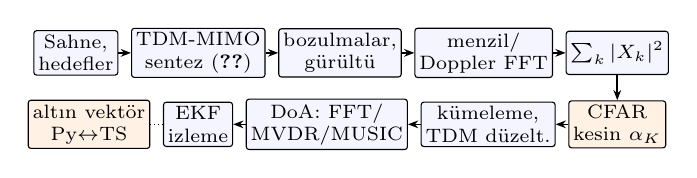
\begin{tikzpicture}[font=\scriptsize, node distance=1.6mm and 1.6mm,
  b/.style={draw, rounded corners=1pt, align=center, inner sep=1.6pt, minimum height=5.5mm, fill=blue!4},
  g/.style={draw, rounded corners=1pt, align=center, inner sep=1.6pt, minimum height=5.5mm, fill=orange!10},
  a/.style={-{Stealth[length=1.3mm]}, semithick}]
\node[b] (s) {Sahne,\\hedefler};
\node[b, right=of s] (y) {TDM-MIMO\\sentez (\ref{eq:beat})};
\node[b, right=of y] (i) {bozulmalar,\\gürültü};
\node[b, right=of i] (f) {menzil/\\Doppler FFT};
\node[b, right=of f] (p) {$\sum_k |X_k|^2$};
\node[g, below=3.2mm of p] (c) {CFAR\\kesin $\alpha_K$};
\node[b, left=of c] (k) {kümeleme,\\TDM düzelt.};
\node[b, left=of k] (d) {DoA: FFT/\\MVDR/MUSIC};
\node[b, left=of d] (t) {EKF\\izleme};
\node[g, left=of t, align=center] (o) {altın vektör\\Py$\leftrightarrow$TS};
\draw[a] (s)--(y); \draw[a] (y)--(i); \draw[a] (i)--(f); \draw[a] (f)--(p); \draw[a] (p)--(c);
\draw[a] (c)--(k); \draw[a] (k)--(d); \draw[a] (d)--(t);
\draw[densely dotted] (o)--(t);
\end{tikzpicture}
\caption{RadarLab işleme zinciri. Python başvuru ve TypeScript (Web Worker) gerçeklemeleri aynı zinciri izler; altın vektörler kapsanan adımlarda iki gerçeklemeyi karşılaştırır.}
\label{fig:chain}
\end{figure}

\textbf{$K$ kanal için kesin CFAR eşiği.} Birim varyanslı karmaşık gürültüde $P$'nin her hücresi $H_0$ altında Gamma$(K,1)$ dağılımlıdır; üstel değildir. CA-CFAR'da eşik $\alpha\,S/N$ olup $S$, $N$ eğitim hücresinin toplamıdır. Test hücresi $X$ için $X/(X+S)\sim\mathrm{Beta}(K,NK)$ olduğundan
\begin{equation}
\begin{aligned}
\Pfa(\alpha)&=1-I_{\alpha/(N+\alpha)}(K,NK),\\
\alpha_K&=\frac{Nu}{1-u},\quad I_u(K,NK)=1-\Pfa
\end{aligned}
\label{eq:alpha}
\end{equation}
elde edilir ($I_u$: düzenlenmiş eksik beta işlevi). Tek kanallı çarpan $\alpha_1=N(\Pfa^{-1/N}-1)$ yalnızca $K=1$ için kesindir. OS, GO ve SO türleri için Gamma sıra istatistiği ve yarım toplam integralleri uyarlamalı sayısal integral ve ikiye bölme yöntemiyle çözülür. Bu sonuçlar klasiktir \cite{shor1991performances,ritcey1990detection}; buradaki katkı denetlenmiş gerçeklemedir.

% =====================================================================
\section{Doğrulama Yöntemi}
Kanıtlar üç sınıfta toplanmıştır. \textbf{(T)~Kurama karşı doğrulama:} simülatör ve işleme zincirinin çıktısı, koddan bağımsız türetilmiş kapalı biçimli bir sonuçla karşılaştırılır. \textbf{(Ö)~Öz-tutarlılık denetimi:} başvuru değeri aynı model ya da koddan gelir; bu denetimler gerilemeleri ve bağlantı hatalarını yakalar, fakat ortak bir modelleme hatasını \emph{yakalayamaz}. \textbf{(A)~Diller arası eşdeğerlik:} Python betiği, girdileri saklanan altın vektör dosyaları üretir; TypeScript test takımı bunları okuyarak ham küpü ($10^{-9}$ bağıl), menzil--Doppler haritasını ($10^{-6}$~dB), dört CFAR türünün eşik ve maskelerini (bağıl $10^{-9}$, sıfır maske farkı, menzil kenarları dâhil), kümelemeyi ve izleyiciyi denetler. Gürültü ve rastgele bozulmalar kapsam dışıdır. Bu karşılaştırmanın gerekliliği bağımsız bir incelemede görülmüştür: iki motor aynı güç haritalarıyla çalıştırıldığında tarayıcı motorunun GO/SO/OS eşiklerinin $K=8$'de tek kanallı formülle hesaplandığı ve 2,6--3,3 kat yüksek olduğu bulunmuş; hata düzeltilmiş ve altın vektörler CFAR eşiklerini kapsayacak biçimde genişletilmiştir. Tablo~\ref{tab:val} doğrulama matrisini özetler; tüm deneyler sabit tohumludur ve tek bir betikle raporlanır.

\begin{table}[!t]
\caption{Doğrulama matrisi (tam Monte-Carlo boyutları). T: kurama karşı, Ö: öz-tutarlılık, GA: güven aralığı.}
\label{tab:val}
\centering\scriptsize
\setlength{\tabcolsep}{2.5pt}
\begin{tabular}{@{}l l l@{}}
\toprule
 & Karşılaştırma & Ölçülen sonuç \\
\midrule
T V1 & CFAR $\Pfa$, 4 tür, $K$=1,4,8 & $|\log_{10}(\hat P/\Pfa)|\leq0{,}028$\\
T V1c & Hann ile $\Pfa$ sapması & ilinti $-0{,}6725$ (kuram $-2/3$)\\
T V2 & $\Pd$, Swerling 0/1/3, $K$=1,8 & 30/30 nokta \%99,9 GA içinde\\
T V3 & RMSE/CRLB: $R$, $v$, $\theta$ & verim 0,956--1,041\\
T V4 & menzil ilintili faz gürültüsü & varyans hatası $-$\%0,95\\
T V5 & iki ışınlı çok yolluluk & sıfır konumu hatası $\leq$\%0,064\\
T V7 & FMCW girişimi & patlama 6 örnek (kuram 6)\\
T V8 & mikro-Doppler & $f_{\max}$ $\pm$1 kutu; kanat $+$\%0,067\\
\midrule
Ö V6 & IQ imge düzeyi & cebirsel özdeşlik\\
Ö V8f & pervane parlama hızı & yapı gereği periyodik\\
Ö V9 & TDM faz düzeltmesi & $-2{,}44\to<0{,}001$ kutu\\
Ö V10 & altın dosyalar (Python) & 13 dosyada sapma 0\\
Ö V11 & .cfg$\to$.bin$\to$işleme & kayıpsız gidiş-dönüş\\
\bottomrule
\end{tabular}
\end{table}

% =====================================================================
\section{Sonuçlar}
\subsection{CFAR yanlış alarm olasılığı}
V1'de dikdörtgen pencereli gerçek FFT gürültü yolundan geçen haritalarda dört CFAR türünün tamamı $K=1,4,8$ için tasarım değerine uymaktadır (durum başına 3\,006\,464 hücre, $\Pfa=10^{-4}$). Tek kanallı çarpan $K$ kanallı toplama uygulandığında eşik $10\log_{10}(\alpha_1/\alpha_K)$ kadar yükselir (Şekil~\ref{fig:cfar}a): $\Pfa=10^{-4}$'te bu fark $K=4$ için 4,07--4,51~dB, $K=8$ için 5,57--6,10~dB'dir ($N=16$--$32$). Gerçekleşen yanlış alarm olasılığı (\ref{eq:alpha})'den $K=4$ için $4\cdot10^{-13}$--$6\cdot10^{-13}$, $K=8$ için yaklaşık $10^{-23}$ düzeyine iner. Dedektör böylece tasarlanandan çok daha tutucu çalışır ve $\Pd=0{,}5$--$0{,}9$ için Swerling~0 hedefte 3,9--7,4~dB, kanallar arasında ilintili Swerling~1 hedefte 4,6--7,4~dB SNR kaybeder. Analitik ifade Monte-Carlo ile de sınanmıştır: $K=8$, $N=40$ ve tasarım $\Pfa=0{,}1$ için tek kanallı çarpanla ölçülen oran $1{,}92\cdot10^{-3}$, (\ref{eq:alpha})'in verdiği değer $1{,}94\cdot10^{-3}$'tür.

\begin{figure}[!t]
\centering
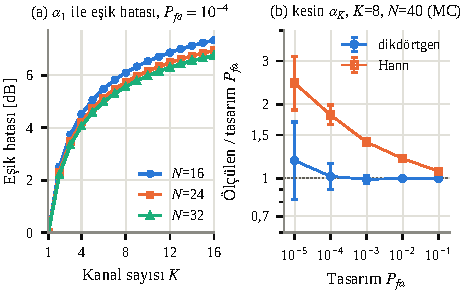
\includegraphics[width=\columnwidth]{figures/fig_cfar_threshold.pdf}
\caption{(a) $K$ kanallı güç toplamında tek kanallı $\alpha_1$ kullanımının eşik hatası. (b) Kesin $\alpha_K$ ile ölçülen/tasarım $\Pfa$ oranı, gerçek FFT gürültü yolu, $K=8$, 2-B CA-CFAR (koruma 1, eğitim 2; $N=40$), 300 harita ($2{,}46\cdot10^6$ hücre), \%95 güven aralıkları.}
\label{fig:cfar}
\end{figure}

\subsection{Hann penceresinin etkisi (V1c)}
Kapalı biçimli CFAR ifadeleri eğitim hücrelerinin bağımsız olduğunu varsayar. Hann penceresi komşu kutular arasında $-2/3$ ilinti yaratır (ölçülen $-0{,}6725$); bu durumda $K=1$, $\Pfa=10^{-3}$ için yanlış alarm oranı CA'da 1,61, OS'de 1,57 kat artmaktadır (dikdörtgen pencerede 1,01 ve 1,03). Şekil~\ref{fig:cfar}b, $K=8$'de etkinin tasarım $\Pfa$ küçüldükçe büyüdüğünü gösterir: oran $10^{-1}$'de 1,07, $10^{-3}$'te 1,40, $10^{-5}$'te 2,44'tür. Hann penceresi yan lob bastırması için çoğu zaman vazgeçilmez olduğundan, bu sapma ya eşik çarpanının Monte-Carlo ile yeniden ayarlanmasını ya da koruma hücrelerinin genişletilmesini gerektirir.

\subsection{Güç toplamı mı, önce hüzmeleme mi?}
Toplama alternatif olarak önce $K$ noktalı açı FFT'si ile hüzmeleme yapılabilir. Birim (üniter) DFT sonrasında her hüzmedeki gürültü yine CN$(0,1)$, yani gücü üsteldir; bu nedenle hüzme başına tek kanallı $\alpha_1$ \emph{doğru} seçimdir. Adil bir karşılaştırma için hüzme başına tasarım olasılığı $1-(1-\Pfa)^{1/K}$ alınmış, böylece hücre başına toplam $\Pfa$ korunmuştur. Monte-Carlo ($K=8$, $d=\lambda/2$, $N=32$, $\Pfa=10^{-4}$, nokta başına $2\cdot10^4$ deneme; yalnız gürültüde $2\cdot10^6$ denemede ölçülen $\Pfa$ toplamda $1{,}05\cdot10^{-4}$, hüzmede $0{,}97\cdot10^{-4}$) sonuçları Şekil~\ref{fig:bf}'de verilmiştir. $\Pd=0{,}9$ için gereken kanal başına SNR, kesin eşikli güç toplamında 5,0~dB, hedef hüzme merkezindeyken hüzmelemede 4,2~dB'dir (kuram; MC: 4,3~dB), yani 0,7--0,8~dB evreuyumlu kazanç vardır. Ancak $\sin\theta$ düzgün dağılımlı olduğunda 5,7~dB, hedef iki hüzmenin tam ortasındayken ise 6,9~dB gerekir. Sıfır doldurmasız hüzmelemenin kazancı, hüzme arası kayıp nedeniyle ortalamada tersine dönmektedir. Tek kanallı çarpanlı güç toplamı ise 10,8~dB ile her iki yaklaşımın da çok gerisinde kalır. Sıfır doldurmalı (aşırı örneklenmiş) hüzmelerde hüzme arası kayıp azalır, ancak hüzmeler ilintili olduğundan toplam $\Pfa$ yeniden ayarlanmalıdır.

\begin{figure}[!t]
\centering
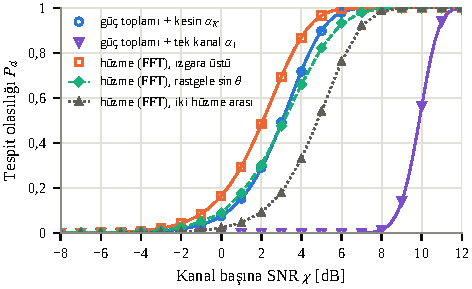
\includegraphics[width=\columnwidth]{figures/fig_beamforming_vs_sum.pdf}
\caption{Swerling~0 hedef, $K=8$, $N=32$, $\Pfa=10^{-4}$: güç toplamı (kesin $\alpha_K$ / tek kanal $\alpha_1$) ve hüzmeleme sonrası hüzme başına CA-CFAR. İşaretler Monte-Carlo, düz çizgiler (\ref{eq:alpha}) tabanlı kuramdır.}
\label{fig:bf}
\end{figure}

\subsection{Tespit olasılığı ve kestirim sınırları}
V2'de tam sentezleyici ve sabit eşikli dedektör, genelleştirilmiş Marcum-Q (Swerling~0) ile kanallar arasında ilintili Swerling~1 ve Swerling~3 kapalı biçimleriyle karşılaştırılmıştır \cite{swerling1960probability,richards2014fundamentals} (Şekil~\ref{fig:valid}a). Önceden belirlenen ölçüt (30 karşılaştırma için Bonferroni tarzı \%99,9 Wilson aralığı) tüm noktalarda sağlanmış; 30 noktanın 29'u \%95 aralığında kalmıştır (nokta başına 3000 deneme). V3'te menzil, hız ve açı, pencerelenmemiş en büyük olabilirlik (ML) ton kestiricisiyle kestirilmiş ve tek karmaşık üstel için CRLB ile karşılaştırılmıştır \cite{rife1974single,kay1993fundamentals}. Örnek başına SNR $-12$~dB ve üzerinde verim (CRLB/MSE) 0,956--1,041 aralığındadır; $-16$~dB'nin altında beklenen eşik etkisi görülmektedir (Şekil~\ref{fig:valid}b). V3 benzetim verisinin doğruluğunu sınar; işleme zincirinin kendisi (Hann penceresi ve log-güç üzerinde parabolik ara değerleme) verimli değildir. Ayrıca TDM-MIMO'da bilinmeyen hız açıyla bağlaştığından açı sınırı bu durumda iyimserdir.

\begin{figure}[!t]
\centering
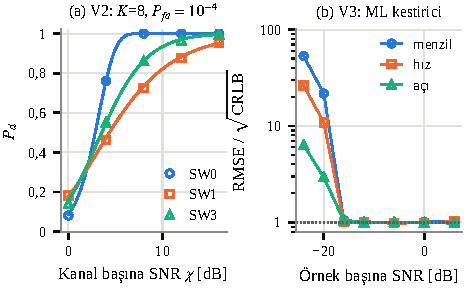
\includegraphics[width=\columnwidth]{figures/fig_validation.pdf}
\caption{(a) V2: $\Pd$ -- SNR, işaretler benzetim, çizgiler kuram. (b) V3: RMSE/$\sqrt{\mathrm{CRLB}}$, 1 Tx $\times$ 4 Rx, $M=16$, $N=32$, SNR başına 2000 deneme.}
\label{fig:valid}
\end{figure}

\subsection{Gerçek veriyle akıl sağlığı denetimi}
Değiştirilmemiş işleme zinciri, herkese açık üç AWR1843 ham ADC kaydına (yaya, bisikletli, park etmiş araç; 30'ar çerçeve) uygulanmıştır \cite{gao2019experiments}. Sıfır Doppler dışında menzil--Doppler gürültüsü Gamma(8) dağılımına uymakta (şekil parametresi 7,88--7,95; KS $p$ 0,17--0,28), kesin $\alpha_K$ ve Hann pencereli CA-CFAR $\Pfa=10^{-3}$'te nominal yanlış alarm oranının 1,12--1,18 katını vermektedir (benzetim: 1,09--1,14). Sıfır Doppler hücreleri ise statik kargaşa ve DC bileşeni nedeniyle modele uymamaktadır ($10^{-4}$'te 10--22 kat). Baskın hedef 0,2~m, 0,08~m/s ve $1^\circ$ içinde yeniden üretilmiştir; ancak yörünge, genlik ve gürültü düzeyi aynı veriye uydurulduğundan bu bir doğruluk testi değil, yalnızca tutarlılık denetimidir.

% =====================================================================
\section{Sonuç}
RadarLab, istatistiksel doğruluğu kapalı biçimli kurama karşı sistematik olarak sınanan ve kurama karşı doğrulamaları öz-tutarlılık denetimlerinden ayıran açık bir FMCW MIMO radar simülatörüdür. Sonuçlar iki pratik uyarı içermektedir: (i) $K$ kanalın güç toplamına tek kanallı CA-CFAR çarpanı uygulanmamalıdır; $K=4$--$8$ için bu hata 4--6~dB'lik eşik ve 3,9--7,4~dB'lik SNR kaybı demektir; (ii) Hann penceresi küçük $\Pfa$ değerlerinde yanlış alarm oranını 2 kattan fazla artırabilir. Önce hüzmelemenin evreuyumlu kazancı ise hüzme arası kayıp nedeniyle ancak hedef hüzme merkezine yakınsa gerçekleşmektedir. Gelecek çalışmalar logaritmik alanda CFAR, sıfır doldurmalı hüzmeleme için eşik ayarı ve kendi donanımımızla köşe yansıtıcı ölçümleridir. Kod ve tarayıcı demosu: \emph{anonim depo}.

% --- Kamera-hazır sürüm: teşekkür ve yapay zekâ kullanım bildirimi (IEEE politikası) ---
% \section*{Teşekkür}
% TODO (yazar): IEEE üretken yapay zekâ politikası gereği kullanılan araçları, sürümlerini ve
% hangi bölümlerde (kod, metin taslağı, şekil betikleri) kullanıldığını burada belirtin.

\bibliographystyle{IEEEtran}
\bibliography{refs}

\end{document}
